\documentclass[11pt]{diazessay} % Font size (can be 10pt, 11pt or 12pt)


\title{\textbf{GW Scattering Calculation Note}} % Title and subtitle

\author{Name: \textbf{Lingyu Xia}} % Author and institution

\date{\today} % Date, use \date{} for no date

\begin{document}

\maketitle

\section{Separation of variables}

Schrödinger's equation in flat space

\begin{align}
    \left(-\frac{1}{2M}\nabla^2-\frac{N_A}{r_A}-\frac{N_B}{r_B}\right)\psi=\epsilon \psi
\end{align}
where $\epsilon$ is the energy of scattering state. Then we use the spheroidal coordinates with 

\begin{align}
    \mu =\frac{r_A+r_B}{R},\quad \lambda =\frac{r_A-r_B}{R},\quad \varphi
\end{align}

As for the d'Alembertian applied on the scalar field $\psi$ is in the form of $\Box \psi=\nabla ^\mu \nabla_\mu \psi$. We first consider situation in flat spacetime, so the covariant operator is equal to partial operator

\begin{align}
    \Box \psi=\nabla ^\mu \nabla_\mu \psi= \partial^\mu \partial _\mu \psi=g^{\mu\nu}\partial_\nu \partial _\mu \psi
\end{align}

Then we calculate the metric of spheroidal coordinate 

\begin{align}
    &r^2_A=x^2+(\frac{R}{2}+z)^2\\
    &r^2_B=x^2+(\frac{R}{2}-z)^2\\
    \implies&\mu=\frac{1}{R}\left(\sqrt{x^2+(\frac{R}{2}+z)^2}+\sqrt{x^2+(\frac{R}{2}-z)^2}\right)\\
    &\lambda=\frac{1}{R}\left(\sqrt{x^2+(\frac{R}{2}+z)^2}-\sqrt{x^2+(\frac{R}{2}-z)^2}\right)
\end{align}

Then we calculate the scale factors

\begin{align}
    &h_\mu=\frac{R}{2}\sqrt{\frac{\mu^2-\lambda^2}{\mu^2-1}}\\
    &h_\lambda=\frac{R}{2}\sqrt{\frac{\mu^2-\lambda^2}{1-\lambda^2}}\\
    &h_\phi=\frac{R}{2}\sqrt{(\mu^2-1)(1-\lambda^2)}
\end{align}

Then we have the Laplacian

\begin{align}
    \nabla^2 \psi= & \frac{1}{\sigma^2\left(\mu^2-\lambda^2\right)}\left\{\frac{\partial}{\partial \mu}\left[\left(\mu^2-1\right) \frac{\partial \psi}{\partial \mu}\right]+\frac{\partial}{\partial \lambda}\left[\left(1-\lambda^2\right) \frac{\partial \psi}{\partial \lambda}\right]\right\} \\ & +\frac{1}{\sigma^2\left(\mu^2-1\right)\left(1-\lambda^2\right)} \frac{\partial^2 \psi}{\partial \varphi^2}
\end{align}
where $\sigma=\frac{R}{2}$.

We introduce the Separation of variables, because $\psi$ in independent of the $\phi$, we separate the $\psi$ in the form of 
\begin{align}
    \psi=\sum_{m}a_m F_m(\mu)G_m(\lambda)e^{im\varphi}
\end{align}

Substitute it into the original equation

\begin{align}
    G_m\partial_\mu \left[(\mu^2-1)\partial_\mu\right]F_m + F_m\partial_\lambda\left[(1-\lambda^2)\partial_\lambda\right]G_m+\notag\\
    \left[-\frac{(\mu^2-\lambda^2)m^2}{(\mu^2-1)(1-\lambda^2)}+2M\mu(N_A+N_B)-2M\lambda(N_A-N_B)+2M\epsilon\sigma^2(\mu^2-\lambda^2)\right]F_mG_m=0\notag
\end{align}

We separate the two variables in the form of $\text{LHS}(\mu,F(\mu))=\text{RHS}(\lambda,G(\lambda))=\rho_m$, then we have

\begin{align}
        {\left[ \dfrac{d}{d\mu} \left( 1-\mu^2 \right) \dfrac{d}{d \mu}+\dfrac{m^2}{1-\mu^2}-\rho_m+2 M \sigma\left(N_A+N_B\right) \mu+2 M \sigma^2 \epsilon\mu^2\right] F_m(\mu)=0}\\
        {\left[\dfrac{d}{d \lambda}\left(1-\lambda^2\right) \dfrac{d}{d \lambda}-\dfrac{m^2}{1-\lambda^2} - \rho_m-2 M \sigma\left(N_A-N_B\right) \lambda-2 M \sigma^2 \epsilon\lambda^2\right] G_m(\lambda)=0}
\end{align}

\section{Power Series Solutions}

We focus on the solutions near the z axis, where $\mu \sim 1$ and $\lambda \in (-1,1)$. Then we could just consider Eq. . On the basis of the Leaver's Eq. 3

\begin{align}
    \frac{d}{d \mu}\left[\left(1-\lambda^2\right) \frac{d G_m}{d \lambda}\right]+\left[-\omega^2 \lambda^2-2 a\left(N_1-N_2\right) \lambda\right. 
    \left.+A_{l m}-m^2 /\left(1-\lambda^2\right)\right] G_m=0
\end{align}
where $\omega=\sqrt{2M\sigma^2 \epsilon}$, $a=M\sigma$, $A_{lm}=\rho_m$.

And then we should transform it into another form. Let $G_m(\lambda)=(1-\lambda^2)^{\frac{m}{2}}g(\lambda)$ 

\begin{align}
    (1-\lambda^2)g_{,\lambda\lambda}-2(m+1)\lambda f_{,\lambda}+\left[\omega^2\lambda^2+2a(N_1-N_2)\lambda+m(m+1)-A_{lm} \right]g=0
\end{align}

On the basis of the work by leaver, we give its power series solutions. First, we should write the standard form for this differential equation. We let $x=\lambda+1$

\begin{align}
    \begin{aligned}
        &x(x  -2) g_{, x x}+2(m+1)(x-1) g_{, x} +\\
        &\left[\omega^2 x(x-2)+2 a\left(N_1-N_2\right)(x-2)\right.  \left.+\omega^2+2 a\left(N_1-N_2\right)+m(m+1)-A_{l m}\right] g=0 .
    \end{aligned}
\end{align}

\begin{align}
    x(x-x_0)\frac{d^2y}{dx^2}+(B_1+B_2x)\frac{dy}{dx}+\left[\omega^2x(x-x_0)-2\eta \omega (x-x_0)+B_3\right]y=0
\end{align}

Following Baber and Hasse, a power series solution about $x=0$ may be obtained by letting 

\begin{align}
    y(x)=e^{i\omega x}\sum_{n=0}^{\infty}a^\theta_nx^n
\end{align}

The sequence of expansion coefficients $\{a^\theta_n:n=1,2,\cdots\}$ is defined by the three-term recurrence relation
\begin{align}
    \begin{aligned}
        &\alpha_0^\theta a_1^\theta&+&\beta_0^\theta a_0^\theta+&=0,&\\
        &\alpha_n^\theta a_{n+1}^\theta&+&\beta_n^\theta a_n^\theta+\gamma_n^\theta a_{n-1}^\theta&=0,&n=1,2, 
    \end{aligned}
\end{align}
where
\begin{align}
    \begin{aligned}
        &\alpha_n^\theta =&-x_0 &n^2+& \left(B_1-x_0\right) n+             &B_1, \\
    &\beta_n^\theta  =&     &n^2+& \left(B_2-2 i \omega x_0-1\right) n+&2 \eta \omega x_0+i \omega B_1+B_3, \\
    &\gamma_n^\theta =&     &    & 2 i \omega n+                       &i \omega\left(B_2-2\right)-2 \eta \omega .
    \end{aligned}
\end{align}

We list the constants in the Eq. 

\begin{align}
    \begin{aligned}
        &B_1=2(m+1),\quad B_2=-2(m+1),\quad B_3=\omega^2+2a(N_1-N_2)+m(m+1)-A_{lm}\\
        &x_0=2,\quad \eta=\frac{2a(N_2-N_1)}{\omega}, \omega=\sqrt{2M\sigma^2 \epsilon}, a=M\sigma, A_{lm}=\rho_m
    \end{aligned}
\end{align}

\section{Numerical Calculation}

\subsection{Power Series Solutions}
Then we use mathematica to calculate numerical solution. We set the $M$ is mass of sun $M=1.9891\times 10^{30}kg$, $R$ is 100 times the diameter of the solar system $R=9\times 10^{12}m$, $\epsilon$ is the energy of incident wave, which satisfies $\epsilon=h\nu=\nu\times 6.62\times 10^{-34}$. Then we use following mathematica's code to plot this power series solution
\newpage

\begin{lstlisting}
    ClearAll[\[Alpha], \[Beta], \[Gamma], F, A]
    \[Alpha][n_] := -2 n^2 + (B1 - 2) n + B1
    \[Beta][n_] := 
     n^2 + (B2 - 4 I \[Omega] - 1) + 4 \[Eta] \[Omega] + I \[Omega] B1 + B3
    \[Gamma][n_] := 
     2 I \[Omega] n + I \[Omega] (B2 - 2) - 2 \[Eta] \[Omega]
    A[0] = 1;
    A[1] = -\[Beta][0]/\[Alpha][0];
    Do[A[n] = (\[Beta][n - 1]*A[n - 1] + \[Gamma][n - 1]*
          A[n - 2])/\[Alpha][n - 1], {n, 2, range}]
    F[x_] := Exp[\[Omega] x] Sum[x^n A[n], {n, 0, range}]
    Plot[{Re[F[x]], Re[F'[x]]}, {x, 0, 0.01}]
\end{lstlisting}

Then, we can use this power series function to get initial condition for original spheroidal equation close to the point A numerically.  We use mathematica's NDSolveValue function to solve spheroidal equation with power series solution's initial condition.

\begin{figure}[ht]
    \centering
    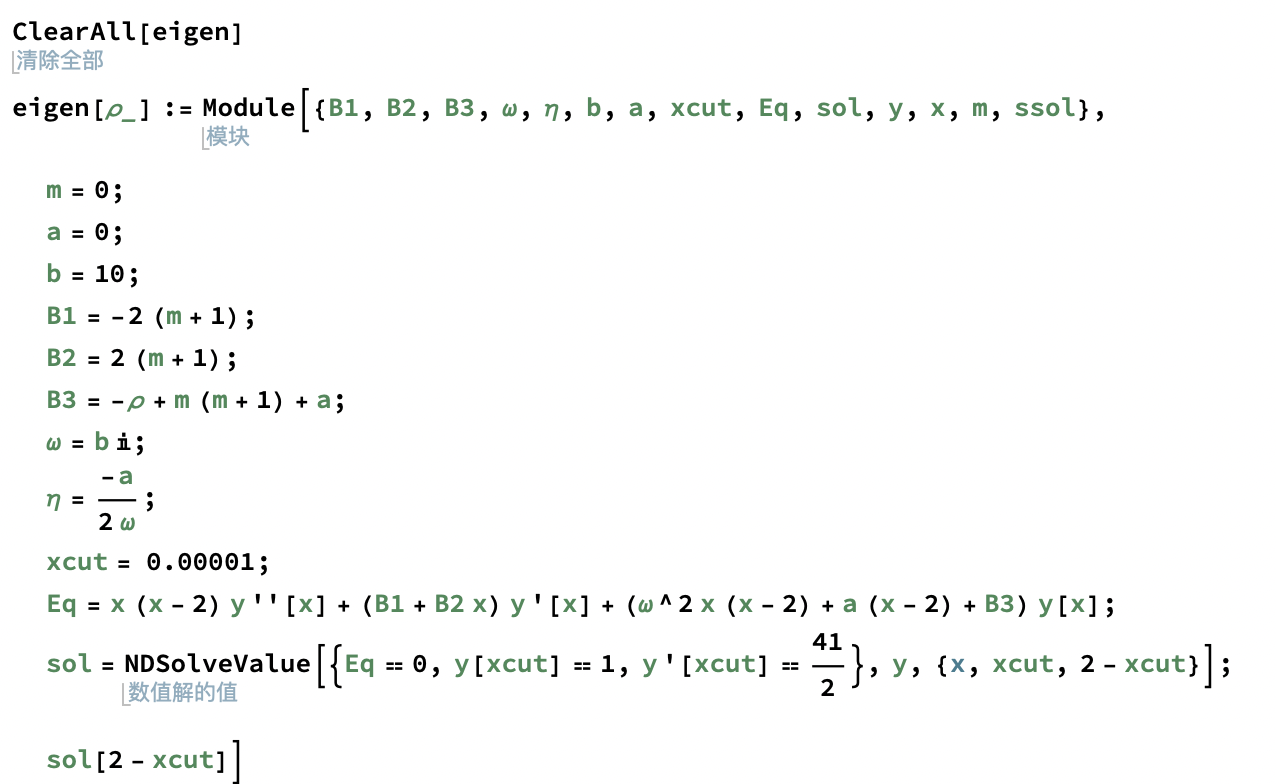
\includegraphics[width=12cm]{6}
\end{figure}

Then we use Interpolation function to fit this solution and plot it in following figure.

\begin{figure}[ht]
    \centering
    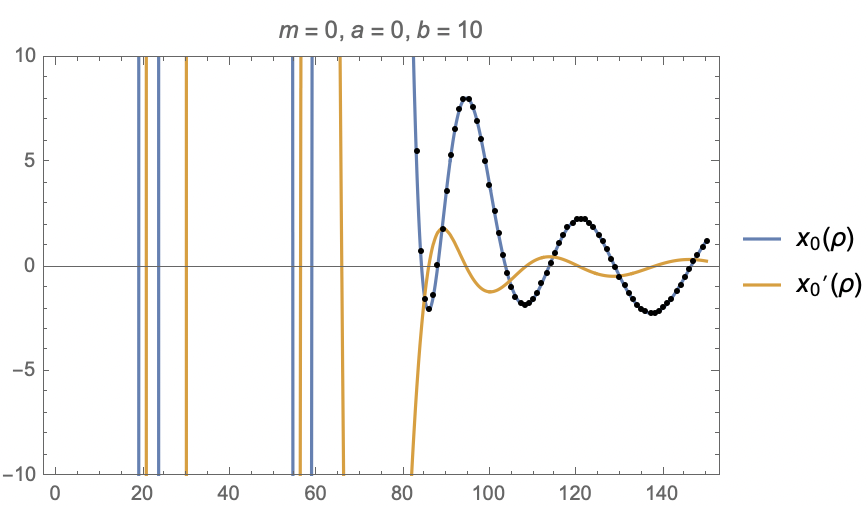
\includegraphics[width=10cm]{5}
\end{figure}

To find the constants from separation variables, we should clarify the criterion that what condition should be satisfied for $\rho$. Obviously, the first derivative of $\lambda$ should be zero at B point, then our criterion is that the first derivative is zero corresponding to the orange line in the above figure. Therefore, we just use function FindRoot to derive the roots. 

\section{Taylor Expansion}

If we consider GW at point B, the effect of point A can be neglected. The partial wave can be expressed by:

\begin{align}
    \int d \rho a_m(\rho) F_m(\rho, \mu) G_m(\rho, \lambda)=\frac{1}{r_A} \sum_l b_{l m} H_l^{A+}\left(x_A\right) \sqrt{\frac{(l-m) !}{(l+m) !}} P_l^m\left(\cos \theta_A\right)
\end{align}

where 

$$x_A=(\lambda+\mu)\sqrt{2M\epsilon}, \quad r_B=\sqrt{r_A^2+R^2-2r_AR\cos\theta_A},\quad \cos\theta_A=\dfrac{1+\lambda\mu}{\lambda+\mu}$$

For a certain partial wave, we have

\begin{align}
    \frac{2}{R(\mu+\lambda)} H_l^{A+}\left(\sqrt{2 M \epsilon} \frac{R}{2}(\mu+\lambda)\right) \sqrt{\frac{(l-m) !}{(l+m) !}} P_l^m\left(\frac{1+\lambda \mu}{\lambda+\mu}\right)=\int d \rho a_{l m}(\rho) F_m(\rho, \mu) G_m(\rho, \lambda)
\end{align}

For line segment $z\in (-\sigma,\sigma)$, $\mu=1$ so the left-hand is nonzero only for $m\neq 0$

\begin{align}
    \frac{1}{\sigma(\mu+\lambda)}\mathcal{F}^{A}_{0}(\omega(\mu+\lambda)) =\int d \rho a_{l 0}(\rho) F_0(\rho, 1) G_0(\rho, \lambda)\label{Formal}
\end{align}

where,

\begin{align}
    \mathcal{F}^{A}_{0}(x) =\frac{e^{-\pi \lambda_A / 2}\left|\Gamma\left(l+1+i \lambda_A\right)\right|}{2(2 l+1) !}(-i)^{l+1} M_{i \lambda_A, l+\frac{1}{2}}(2 i x)=\frac{1}{2 i}\left[H_l^{A+}(x)-H_l^{A-}(x)\right]
\end{align}

Then we expand both sides of equation, and align the term of $(1+\lambda)$ order by order. The Taylor expansion can be obtained in Leaver's paper. For the case of m = 0, one has,

\begin{align}
    G_0(\rho, \lambda)=e^{i \omega(\lambda+1)}\sum_{n=0}^{+\infty}c^{\lambda}_{n}(\rho)(\lambda+1)^{n}
\end{align}

\begin{align}
    \begin{aligned}
        &\alpha_0^\theta c_1^\theta&+&\beta_0^\theta c_0^\theta+&=0,&\\
        &\alpha_n^\theta c_{n+1}^\theta&+&\beta_n^\theta c_n^\theta+\gamma_n^\theta c_{n-1}^\theta&=0,&n=1,2, \cdots 
    \end{aligned}
\end{align}

where

\begin{align}
    \begin{array}{l}
    \alpha_n^\lambda=-2 n^2-\left(B_2+2\right) n-B_2, \\
    \beta_n^\lambda=n^2+\left(B_2-4 i \omega-1\right) n-a-i \omega B_2+\rho+m(m+1), \\
    \gamma_n^\lambda=2 i \omega n+i \omega\left(B_2-2\right)+a,
    \end{array}
\end{align}

and, 

\begin{align}
    \begin{aligned}
    a & =2 M \sigma\left(N_A-N_B\right)=-2 \omega\left(\lambda_A-\lambda_B\right), \\
    B_2 & =2(m+1) .
    \end{aligned}
\end{align}

Assume that $c^{\theta}_{0}=1$, and we can calculate each term for $c^{\theta}_{\lambda}$

\begin{align}
    \begin{aligned}
    c_1^\lambda & =\frac{\rho}{2}-\frac{1}{2}(a+2 i \omega) \\
    c_2^\lambda & =\frac{1}{16} \rho^2+\frac{1}{8}(1-a-4 i \omega) \rho+\frac{1}{16}\left(a^2+8 i a \omega-12 \omega^2\right)\\
    c_3^\lambda & =\frac{1}{288} \rho^3+\frac{1}{288}(8-3 a-18 i \omega) \rho^2+\frac{1}{288}\left(3 a^2+36 i a \omega-6 a-92 \omega^2-36 i \omega+12\right) \rho \\
    & -\frac{1}{288}\left(a^3+18 i a^2 \omega+2 a^2-92 a \omega^2-120 i \omega^3+8 \omega^2\right)\\
    &\cdots 
    \end{aligned}
\end{align}

Then we define "\textit{n}th moment" as, 

\begin{align}
    Z_{n}=\int d \rho a_{l0}(\rho)F_{0}(\rho, \mu)\rho^{n}
\end{align}

Thus, Eq. (\ref{Formal}) 

\begin{align}
    \begin{aligned}
        e^{i \omega(\lambda+1)}&\left\{Z_0+\frac{1}{2}(\lambda+1)\left[-(a+2 i \omega) Z_0+Z_1\right]\right. \\
    &+\frac{1}{16}(\lambda+1)^2\left[\left(a^2+8 i a \omega-12 \omega^2\right) Z_0+2(1-a-4 i \omega) Z_1+Z_2\right] \\
    &+\frac{1}{288}(\lambda+1)^3\left[-\left(a^3+18 i a^2 \omega+2 a^2-92 a \omega^2-120 i \omega^3+8 \omega^2\right) Z_0\right. \\
    &\left.+\left(3 a^2+36 i a \omega-6 a-92 \omega^2-36 i \omega+12\right) Z_1+(8-3 a-18 i \omega) Z_2+Z_3\right] \\
    &\left.+\mathcal{O}\left((\lambda+1)^4\right)\right\} \\
    \end{aligned}
\end{align}

And we can use Mathematica to expand LHS of Eq.(\ref{Formal}) to obtain each moment



\section{NEW THOUGHTS WITH TAYLOR EXPANSION}

For $m=0$ wave at $\lambda \rightarrow-1$, we have,
\begin{align*}
\frac{1}{\sigma(\mu+\lambda)} H_0^{A+}(\omega(\mu+\lambda))=\int d \rho a_0(\rho) F_0(\rho, \mu) G_0(\rho, \lambda)
\end{align*}
$[\mathrm{lx}, \mathrm{hz}]$ where $\omega=\sqrt{2 M \epsilon} \sigma$ and $H_l^{A \pm}(x)$ is defined as,
\begin{align*}
\frac{\partial^2}{\partial x^2} H_l^{A \pm}(x)+\left[1-\frac{l(l+1)}{x^2}-\frac{2 \lambda_A}{x}\right] H_l^{A \pm}(x)=0 .
\end{align*}
[lx,hz] Comparing to Eq. (1), one has,
\begin{align*}
\begin{aligned}
x & =\omega r_A / \sigma, \\
\lambda_A & =-\sqrt{\frac{M}{2 \epsilon}} N_A .
\end{aligned}
\end{align*}
[lx] The $H_l^{A \pm}$ can be written in terms of Whittaker functions,
\begin{align*}
H_l^{A \pm}(x)=(\mp i)^l e^{\left(\pi \lambda_A / 2\right) \pm i \sigma_l\left(\lambda_A\right)} W_{\mp i \lambda_A, l+\frac{1}{2}}(\mp 2 i x),
\end{align*}
$[\mathrm{lx}, \mathrm{hz}]$ where,
\begin{align*}
\sigma_l\left(\lambda_A\right)=\arg \left(\Gamma\left(l+1+i \lambda_A\right)\right)
\end{align*}
[lx,hz] The \pm sign labels the asymptotic behaviour of the solution,
\begin{align*}
H_l^{A \pm}(x) \rightarrow e^{ \pm i\left[x-\lambda_A \log (2 x)-\frac{l}{2} \pi+\sigma_l\left(\lambda_A\right)\right]} .
\end{align*}
[lx,hz]
However, Eq. (6) has a severe flaw. The LHS diverges at $A$. A more realistic calculation should be,
\begin{align*}
\frac{1}{\sigma(\mu+\lambda)} \mathcal{F}_0^A(\omega(\mu+\lambda))=\int d \rho a_0(\rho) F_0(\rho, \mu) G_0(\rho, \lambda)
\end{align*}



\end{document}